\section{Core Components}
\label{chp5::sec::taxonomy}

\subsection{Taxonomy of Password Guessing Strategies}

At a high level, we categorise password guessing attack strategies based on the guess rate and knowledge of the target. The guess rate is determined by whether the attacker has the hash value or not, which also determines whether the attack is offline or online. \textit{An offline attack} assumes unlimited guessing attempts, while an online attack is typically rate-limited by the target application (we assume we do not possess the hash value). The second factor is whether the attack is targeted, assuming knowledge about the target (e.g., personal information and previous passwords). Figure~\ref{fig:attack-types} illustrates these factors and their relationships.

\begin{itemize}
\item \textbf{Offline Attacks.} In situations where adversaries have access to password hash values, they are able to make unlimited attempts to guess the passwords without restriction.

\item \textbf{Online Attacks.} Conversely, guessing attempts are restricted by security protocols implemented within the target applications.
\end{itemize}

\begin{figure}
\centering
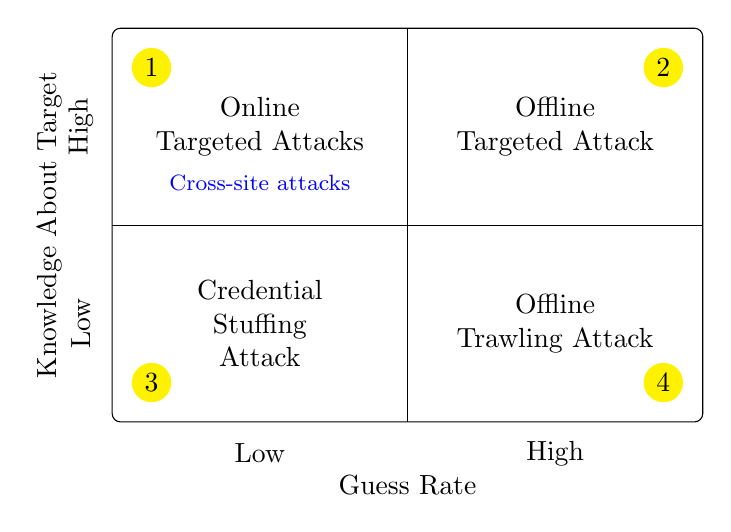
\begin{tikzpicture}
    % Variables for the grid size
    \def\gridwidth{7.5}
    \def\gridheight{5}

    % Draw the main grid
    \draw[rounded corners=3pt] (0,0) rectangle (\gridwidth,\gridheight);
    
    % Draw the dividing lines
    \draw (\gridwidth/2,0) -- (\gridwidth/2,\gridheight);
    \draw (0,\gridheight/2) -- (\gridwidth,\gridheight/2);
    
    % Labels for the attack types
    \node[align=center] (box1) at (\gridwidth/4,3*\gridheight/4) {Online\\Targeted Attacks};
    \node[align=center] at (3*\gridwidth/4,3*\gridheight/4) {Offline\\Targeted Attack};
    \node[align=center] at (\gridwidth/4,\gridheight/4) {Credential\\Stuffing\\Attack};
    \node[align=center] at (3*\gridwidth/4,\gridheight/4) {Offline\\Trawling Attack};

    \node[below, text=blue, font=\footnotesize] at (box1.south) {Cross-site attacks};
    
    % Labels for the axes
    \node[align=center] at (\gridwidth/2,-0.8) {Guess Rate};
    \node[align=center, rotate=90] at (-0.8,\gridheight/2) {Knowledge About Target};
    
    % Axis numbers
    \node[align=center] at (\gridwidth/4,-0.4) {Low};
    \node[align=center] at (3*\gridwidth/4,-0.4) {High};
    \node[align=center, rotate=90] at (-0.4,3*\gridheight/4) {High};
    \node[align=center, rotate=90] at (-0.4,\gridheight/4) {Low};


    % Circles with numbers
    % Upper left
    \node[circle,fill=yellow,inner sep=0pt,minimum size=0.5cm] at (0.5,\gridheight-0.5) {1};
    % Upper right
    \node[circle,fill=yellow,inner sep=0pt,minimum size=0.5cm] at (\gridwidth-0.5,\gridheight-0.5) {2};
    % Lower left
    \node[circle,fill=yellow,inner sep=0pt,minimum size=0.5cm] at (0.5,0.5) {3};
    % Lower right
    \node[circle,fill=yellow,inner sep=0pt,minimum size=0.5cm] at (\gridwidth-0.5,0.5) {4};

\end{tikzpicture}
\caption{Categories of attacks based on the attack rate (available to the attacker) on the horizontal axis and the amount of knowledge the attacker has about the target on the vertical axis. High attack rate signifies that the attacker has access to the target's hash. A low attack rate means that the attacker is trying to attack a hash through a rate limited service.}
\label{fig:attack-types}
\end{figure}

\begin{figure}[h]
    \centering
    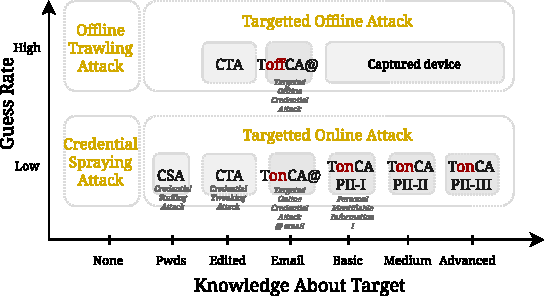
\includegraphics[scale=1.5]{figs/how_passwords/classification_of_strategy.pdf}
    \caption{Detailed representation of algorithms conditioned on guess rate and the type of information is used for targeting.}
    \label{fig::chp5::knowledge-attack-matrix}
\end{figure}

The contextual information used for targeting can be further broken down into categories that have been inspired by previous studies~\cite{pal_beyond_2019, wang_pass2edit_2023, wang_password_2023, wang_targeted_2016}. These studies have shown that using contextual information (such as previous passwords or PII) improves the likelihood of guessing human-chosen and memorable secrets. Figure~\ref{fig::chp5::knowledge-attack-matrix} visualises the detailed breakdown of contextual information with respect to the guess rate. This is summarised in Conjecture~\ref{conjecture::chp5::contextual-info}---Our analysis of the content of the password, especially the location information, showed how users embed information about themselves and environment into their secrets.

\begin{conjecture}[PII and Knowledge Embedding in Secrets]
When a person creates a secret (such as a password), they naturally embed information from their personal context into it. This embedding follows predictable patterns based on different categories of contextual information, including personal, environmental, temporal, social, and behavioural information. The likelihood of finding patterns derived from any particular type of contextual information in the secret increases with both the psychological proximity that the information has to the person and the ease with which it makes the secret memorable. This embedding occurs at a rate significantly higher than what would be expected by chance, with the strength of embedding varying based on how cognitively accessible and personally relevant the contextual information is to the creator.
\label{conjecture::chp5::contextual-info}
\end{conjecture}


\noteBox{Research Opportunity}{%
Given a limited set of strategically chosen questions about a user and their truthful answers, it is possible to generate a relatively small set of candidate passwords that contains the user's actual password with probability significantly higher than random guessing. This is achievable if and only if the questions are specifically designed to reveal information about how the user incorporates personal information into their passwords and their password creation habits. The resulting set of candidate passwords will be substantially smaller than the set of all possible passwords of the same length and character composition.
}

Conditioning a guess on assumptions about the content or structure of the password also affects guessing performance. Techniques like masking have proven highly useful in practice.

Some literature may categorise their method as a \textit{Cross-site attack}; in the context of their use, this means that the attack is targeted and uses breached passwords from other websites (hence the name cross-site). However, this strategy is often known as \textit{Credential Stuffing Attack}. If further targeting occurs, i.e., editing the password, then we call this \textit{Credential Tweaking Attack}.

Beyond credential tweaking attack, one may use more Personally Identifiable Information (PII) such as email address, date of birth, family information, and etc. As shown in Figure~\ref{fig::chp5::knowledge-attack-matrix}, we refer to these as \textbf{T}argeted \textbf{on}line \textbf{CA} (Credential Attack).

These high level strategies aim to capture the environmental limitations. There are further limitations imposed within each category, e.g. a memory-hard hash function might demand a different strategy to a simpler hash function. Also, these strategies thus far have not captured the \textit{mode} of the attack; this is the aim of the next section.

\begin{figure*}[]
    \centering
    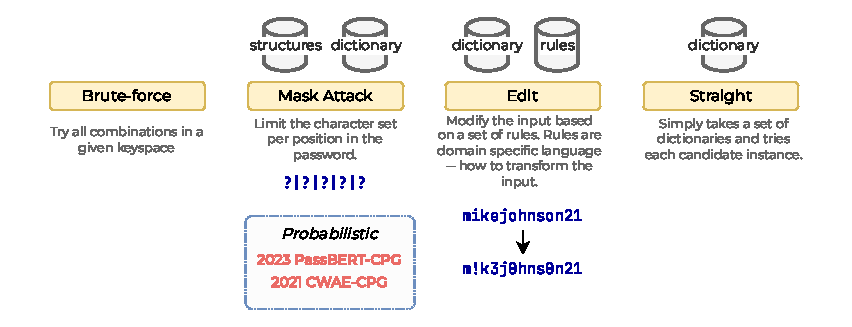
\includegraphics[scale=1.1]{figs/how_passwords/modes_passwords.pdf}
    \caption{Examples of mode of attack.}
    \label{fig::chp5::modes-of-attack}
\end{figure*}

\subsection{Generation Modes}
\label{sec::chp5::modes}

Password guessing algorithms are essentially generative functions. These algorithms can be classified into three main categories: probabilistic, deep learning-based, and deterministic (or rule-based) approaches~\cite{yu_systematic_2023, tran_survey_2022}. However, this classification is overly simplistic for practical applications. Instead, we propose categorizing password guessing algorithms based on their \textbf{mode} of attack, which better reflects their real-world effectiveness and implementation. Some of these modes are illustrated in Figure~\ref{fig::chp5::modes-of-attack}.

In academic research, most password guessing methods operate as \textit{dictionary generators}, where the primary focus is on generating potential password candidates. The actual password cracking process typically relies on established tools such as \hashcat or John the Ripper (JtR)~\cite{JtR}, which perform the hash comparison operations. These open-source tools are highly optimized to take advantage of many types of GPUs and architectures to speed up the hashing process.

\begin{definition}[Dictionary/Wordlist]
A collection of precomputed password candidates, typically containing:
\vspace{-15pt}
\begin{itemize}
\setlength{\itemsep}{-5pt}
    \item Common passwords from data breaches
    \item Words from natural languages
    \item Known password patterns
    \item Organization-specific terms
    \item Common keyboard patterns and variations
\end{itemize}
\end{definition}

The concept of attack \textbf{modes} is largely influenced by Hashcat's implementation architecture. Hashcat, together with JtR, has established itself as the industry standard for offline password cracking, offering various attack strategies optimized for different scenarios and password patterns. This mode-based approach provides a more practical framework for understanding and implementing password guessing algorithms.

\begin{itemize}
    \item \textbf{Brute-force}: In this mode, we try all combinations in a character space. This mode is essentially obsolete for any useful password guessing.
    
    \item \textbf{Mask attack}: An attacker reduces the number of combinations to try by limiting which characters can appear in each position of the password. This approach works well when the attacker knows part of the password structure. Section \ref{sec::chp5::mask-attack} explains mask attacks in detail and conducts a systemisation of the mode.
    
    \item \textbf{Edit}: An attacker modifies existing password candidates using specific rules. In Hashcat, these rules tell the programme exactly how to alter each candidate password.

    \item \textbf{Straight}: An attacker attempts passwords using a set list. \hashcat refers to this method as a \textit{Straight} attack. When attackers merge multiple dictionaries, it is termed a \textit{Combinator} attack.
    
    \item \textbf{Generative}: Attackers can generate new password candidates using several methods:
    
    \begin{itemize}
        \item \textbf{Markov n-gram models}: These analyse how frequently certain character sequences appear and use those patterns to generate likely passwords. Password crackers widely use this effective approach.
        
        \item \textbf{Probabilistic Context-Free Grammar (PCFG)}: This method creates rules on the password structure and assigns probabilities to each rule. PCFGs excel at generating passwords that look like those created by humans.
        
        \item \textbf{Deep Learning}: Networks like RNNs and GANs learn patterns from leaked password databases to generate similar passwords. As more password databases become public, researchers increasingly use deep learning to crack passwords.
        
        \item \textbf{Machine Learning}: Algorithms like decision trees, random forests, and support vector machines help attackers predict which passwords to try first.
    \end{itemize}
    
    \item \textbf{Hybrid}: An attacker combines multiple methods above to create more sophisticated attacks. For example, combine dictionary attack with mask attack.
\end{itemize}

Although these modes and password guessing attacks are presented as distinct categories, they are better approached as overlapping characteristics. For example, a generative model such as \cwaecpg using deep learning incorporates mask-like constraints. Therefore the modes and categorisations aren't mutually exclusive.

Ideally we should be able to chain these functions together and condition them on available information. The output of one function can serve as the input to another, creating a more sophisticated attack pipeline.

\subsection{Existing Algorithms}

\begin{table}[h]
%\footnotesize
\centering
\begin{tabular}{crlll}
\toprule
\textbf{Year} & \textbf{Model} & \textbf{Data} & \textbf{Comparison} & \textbf{Method} \\
\midrule
2023 & \rfguess & \begin{tabular}[c]{@{}l@{}}Rockyou\\ 000webhost\end{tabular} & \begin{tabular}[c]{@{}l@{}}FLA\\ PCFG\\ Markov\end{tabular} & \begin{tabular}[c]{@{}l@{}}Random\\ Forest Trees\end{tabular} \\
\hdashline
2022 & \gnpassgan & \begin{tabular}[c]{@{}l@{}}Rockyou\\ phpbb\end{tabular} & PassGAN & GAN \\
\hdashline
2022 & \omecdn & \begin{tabular}[c]{@{}l@{}}Rockyou\\ Yahoo\\ 12306\\ CSDN\end{tabular} & \begin{tabular}[c]{@{}l@{}}OMEN\\ PassGAN\end{tabular} & \begin{tabular}[c]{@{}l@{}}Markov\\ n-gram\end{tabular} \\
\hdashline
2021 & \adams  & 4iQ & \begin{tabular}[c]{@{}l@{}}Hashcat\\ Markov\end{tabular} & ANN \\
\hdashline
2019 & \passgan & \begin{tabular}[c]{@{}l@{}}Rockyou\\ LinkedIn\end{tabular} & \begin{tabular}[c]{@{}l@{}}Hashcat\\ PCFG\\ FLA\\ JtR\end{tabular} & GAN \\
\hdashline
2016 & \fla & \begin{tabular}[c]{@{}l@{}}PGS\\ PGS++\end{tabular} & \begin{tabular}[c]{@{}l@{}}PCFG\\ JtR\\ Hashcat\end{tabular} & LSTM \\
\hdashline
2015 & \omen & \begin{tabular}[c]{@{}l@{}}Rockyou\\ MySpace\\ Facebook\end{tabular} & \begin{tabular}[c]{@{}l@{}}Markov\\ PCFG\\ JtR\end{tabular} & \begin{tabular}[c]{@{}l@{}}Markov\\ n-gram\end{tabular} \\
\hdashline
2009 & \pcfg & \begin{tabular}[c]{@{}l@{}}MySpace\\ Finnish List\\ SilentWhisper\end{tabular} & JtR & PCFG \\
\hdashline
2005 & \markovngram & 142 Passware & Rainbow Table & \begin{tabular}[c]{@{}l@{}}Markov\\ n-gram\end{tabular} \\
\bottomrule
\end{tabular}
\caption{Examples of trawling and non-targetted password guessing methods and algorithms.}
\label{tab:password_analysis}
\end{table}


\subsubsection{PRINCE Algorithm}
The PRINCE algorithm \cite{princeprocessor2015} (\textbf{PR}obability \textbf{IN}finite \textbf{C}hained \textbf{E}lements''), is a password guessing algorithm when given an input wordlist $W$ and a target length $n$, the algorithm generates password candidates through permuted combinations. The algorithm was introduced by Jens Steube in 2014.

\subsubsection{Probabilistic Algorithms}

\textbf{Markov $\bm{n}$-gram} \cite{narayanan_fast_2005}. Markov $n$-gram models have been widely used for password guessing, with numerous iterations and improvements over time. The basic idea behind Markov $n$-gram models is to capture the statistical properties of passwords by analysing the frequency and probability of character sequences.

One notable example is \omen which outputs password guesses in descending order of their likelihood--prioritizing more probable passwords. This approach allows for more efficient password guessing by focusing on the most promising candidates first.

Building upon \omen, \omecdn incorporates a neural network-based discriminator to rank and filter the generated passwords. The discriminator, denoted as $f_{\text{GAN-D}}$, assigns a score $S$ to each password:
\begin{equation}
S = f_{\text{GAN-D}}(X)
\end{equation}
\omecdnnocite\ then selects a subset of passwords $D_{\text{OMECDN}}$ from the OMEN-generated passwords $D_{\text{OMEN}}$ based on a threshold $\gamma$:
\begin{equation}
D_{\text{OMECDN}} = { X \in D_{\text{OMEN}} : f_{\text{GAN-D}}(X) \geq \gamma }
\end{equation}
While \omecdnnocite\ provides a marginal improvement over \omennocite\ (4.07\%), it likely introduces a significant overhead in terms of generation speed compared to \omennocite.

The performance of Markov $n$-gram models can be further enhanced by incorporating additional techniques, such as smoothing and interpolation, to handle unseen or rare character sequences. Smoothing methods, such as Laplace smoothing or Kneser-Ney smoothing, assign non-zero probabilities to unseen $n$-grams, preventing the model from assigning zero probability to potentially valid passwords.

Interpolation techniques, such as linear interpolation or backoff, combine the probabilities of different order $n$-grams to improve the model's ability to handle novel sequences. For example, linear interpolation computes the probability of an $n$-gram as a weighted sum of the probabilities of lower-order $n$-grams:

% \begin{equation}
% P(x_i | x_{i-n+1}^{i-1}) = \sum_{k=1}^{n} \lambda_k P_k(x_i | x_{i-k+1}^{i-1})
% \end{equation}
% where $P_k$ denotes the probability of an $n$-gram of order $k$, and $\lambda_k$ are the interpolation weights, satisfying $\sum_{k=1}^{n} \lambda_k = 1$.

\textbf{Probabilistic Context-Free Grammar}. \pcfg\ models represent password structures as a set of grammar rules with associated probabilities. By learning the grammar from a password dataset, \pcfgnocite\ models can generate password guesses that adhere to the learned patterns and structures. The model works by dividing passwords into chunks based on letters ($L$), digits $D$, and special symbols $S$. The model then learns the rules and probabilities for these chunks from a training dataset. For example, this is how a password is represented in the \pcfgnocite\ grammar:
\[
\text{\password{password22!}} \rightarrow L_8D_2S_1
\]
Subsequent variants of the original \pcfg\ have introduced key improvements. \wordpcfg\ introduces word extraction techniques to identify semantic segments, including dictionary words, keyboard patterns, and other combinations, rather than only relying on basic character classes. \personalpcfg\ expanded the symbol sets to include semantic categories like birthdates, names, and personal information, enabling more targeted password guessing. Probability assignment has been refined by using frequency-based probabilities and non-zero probabilities for unseen strings, with some models also using cross-validation to improve generalisation. Finally, hybrid models, such as \passtcn, have been developed that integrate \pcfgnocite\ with other methods, like Markov models and Recurrent Neural Networks.

\noteBox{Research Opportunity}{%
A 2014 comprehensive review of probabilistic models by Ma et al. \cite{ma_study_2014} concludes that whole string Markov models generally outperform \pcfgnocite models in password guessing tasks. This finding suggests that capturing the statistical properties of entire passwords is more effective than modelling the underlying grammar structure. With the improvements of the original \pcfg model, and perhaps using different algorithms and architectures, it would be interesting to see whether that conclusion remains valid.
}
\vspace{-0.25cm}
\subsubsection{Deep Learning}

\fla\ was one of the first methods to use an LSTM network to model passwords and show that they can be competent and at times superior to the likes of \markovngramnocite and \pcfgnocite-based models; particularly for non-traditional password policies and when making more than $10^{10}$ guesses. Interestingly, the model did not have a material benefit from natural language dictionaries in the training set. However, an extended experiment might attempt this with different natural languages. For example, how would the results differ if the training set is in English but the test set is in Spanish?
% \fla created a larger model using c.60MB of space for offline attack and a smaller model of c.2.7MB for client-use.

\passgan\ uses a Generative Adversarial Network (GAN) to learn the distribution of real passwords from actual password leaks. Results show that it is competitive with state-of-the-art password guessing algorithms, and it can augment password generation rules by matching passwords that were not generated by other rules-based methods. There have been incremental improvements over the original \passgannocite\ model. \passgannocite\ used an Improved Wasserstein GAN (IWGAN) with gradient penalty. Subsequent models like \gnpassgan\ addressed these issues by adopting gradient normalisation on the discriminator, which imposes a gradient norm restriction, and using binary entropy loss with a sigmoid layer instead of the Wasserstein loss. This approach enhanced the discriminator's capacity, reduced mode collapse, and led to better guessing capabilities and reduced duplicate password generation.

Other improvements include changes to the network architectures. \redpack\ replaced the ResNet blocks in \passgannocite\ with Recurrent Neural Networks (RNNs), introducing a new cost function for greater stability. \gpass\ uses LSTM in the generator for better sample quality, and multiple convolutional layers with varying filter sizes in the discriminator. \gpassnocite\ also incorporates Gumbel-Softmax with temperature control, allowing for a trade-off between sample diversity and quality by adjusting the temperature during training. \cwaegan\ introduces stochastic smoothing to the password representation, which allows for more training iterations and greater model stability. The model also employs a deeper network architecture with residual bottleneck blocks and batch normalisation, which improves its ability to learn complex password patterns, leading to a higher matching rate compared to \passgannocite.

The Adaptive Dynamic Mangling rules attack (\adams) is an adaptation of Hashcat's mangling/edit mode. \adamsnocite\ aims to adapt to the target password distribution at runtime by learning best mangling rules rather than relying on static, pre-configured rules. \adamsnocite\ seems more efficient, i.e. less guesses required for a successful crack. \adamsnocite\ outperforms the standard mangling mode. Though, here the quality of the rule-set used is highly important and would have a material effect on the outcome of the experiment.

% In summary, Markov $n$-gram models have proven to be effective in password guessing tasks, with various improvements and extensions proposed over time. While PCFG models offer an alternative approach, whole string Markov models have generally demonstrated superior performance. The effectiveness of Markov $n$-gram models can be further enhanced through techniques such as smoothing and interpolation, making them a powerful tool for password guessing and security analysis.

%\textbf{RFGuess} \cite{wang_password_2023} (2023) uses Random Forest trees to generate passwords. The authors have falsely called this trawlling attack, the two algorithms sit between \textit{Credential Stuffing Attack} and \textit{Online Targeted Attack}. The authors claim that is similar to the Markov 7-gram model without much comparison to the Markov 7-gram models in the results section. They compare the model to PCFG, Markov and FLA. Experiment scenarios are split between different sites (cross-sites) and inter-site, where they use a portion of the leaked password set to the training and the remaining portion for testing. RFGuess uses the Rockyou and 000webhost dataset for the trawling attack. The results are inconclusive in our opinion. With a lack of tabular data it is difficult to judge the differences in the models. The different graphs show RFGuess performing similar to worse than its counterparts. The claim that \emph{`RFGuess outperforms all its counterparst in intra-site guessing scenarios'} can not be seen in the results. Lastly, the authors falsely claim that RFGuess is suitable for online password guessing scenarios. The results (in Fig 6 and 7 in their paper) invalidates this statement. Their claim that online guessing is unavoidable and its success is rather high is also false. Majority of websites implement rate limiting in their authentication systems. In summary, the use of Random Forest Trees for trawling attack is inconclusive from this paper and the results are deemed to be worse than their counterparts.
%
%\textbf{PassBERT} \cite{xu_improving_2023} introduces three distinct attack methodologies: Conditional Password Guessing (CPG), Targeted Password Guessing (TPG), and Adaptive Rule-based Password Guessing (ARPG). This study focuses primarily on the non-targeted trawling attack, namely CPG. The data pre-processing phase involves the exclusion of hashed passwords, the elimination of non-ASCII character passwords, and the removal of passwords exceeding 32 characters in length. Passwords undergo tokenization at the character level, incorporating the {[}CLS{]} and {[}SEP{]} tokens to signify the commencement and termination of sequences, respectively. The model's pre-training employs the Rockyou-2021 dataset, utilizing a random sampling of 60 million entries. On average, PassBERT demonstrates a password generation rate of 4.54 passwords per second. A comparative analysis is conducted with the Context Wasserstein Autoencoder (CWAE) as documented in Pasquini et al.~(2021)  \cite{pasquini_improving_2021}. Notably, the referencing of this model appears to be erroneous. The rationale provided by the authors for selecting CWAE over Pass2path (Pal et al., 2019) \cite{pal_beyond_2019} and ADaMs (Pasquini et al., 2021) \cite{pasquini_reducing_2021} is predicated on CWAE's superior performance. The reproducibility of password guessing attacks presents significant challenges. Efforts to contact the original authors for access to the model and its weights proved futile, further complicating the replication process.
%
%\textbf{CWAE} \cite{pasquini_improving_2021} This paper proposes using representation learning with deep generative models like GANs and autoencoders for password guessing. The authors train these models on leaked password datasets like RockYou to learn a latent representation of passwords that captures semantic relationships. They introduce two novel password guessing frameworks - Conditional Password Guessing (CPG) which can generate biased guesses, and Dynamic Password Guessing (DPG) which adapts the guessing strategy based on successfully guessed passwords. CPG allows generating passwords matching arbitrary templates or biases using the strong locality property of the latent space. DPG leverages the weak locality to reduce the covariate shift between train and test password distributions. The authors compare these techniques against probabilistic guessers like OMEN, PCFG and FLA on biased test sets created from LinkedIn data. They show CPG can efficiently generate rare biased guesses unlike other methods. DPG adapts and outperforms static attacks on diverse leaks like Youku and Zomato exhibiting distribution shifts.

%\textbf{PASS2EDIT} (2023) \cite{wang_pass2edit_2023} introduces a new approach for guessing edited passwords in targeted attacks by modelling password tweaking as a multi-class classification problem. The authors propose a multi-step decision-making mechanism combined with a generative model to characterize users' password reuse and modification behaviours. They evaluate PASS 2 EDIT using 12 attack scenarios and a large dataset of 4.8 billion passwords.
%The paper claims that PASS 2 EDIT outperforms prior methods such as Pass2Path and TarGuess-II, achieving 18.2\%-33.0\% higher cracking success rates within 100 guesses when the victim's password at one site is known. However, the evaluation relies heavily on the specific attack scenarios and datasets chosen, and the generalizability of the results to other settings is unclear.
%While the authors emphasize the severity of password tweaking threats, the practical impact may be less significant than suggested, as the success rates are still relatively low even with PASS 2 EDIT. Moreover, the paper does not adequately address the limitations of the proposed approach or discuss potential countermeasures.
%Overall, PASS2EDIT offers a new perspective on characterizing password reuse behaviours but falls short of providing a comprehensive understanding of users' password security. The claims of superiority over prior art should be interpreted with caution, as the evaluation is limited in scope and may not reflect real-world performance in diverse settings.

\subsection{Limitations of Existing Methods}
Current methods do not incorporate the speed of generation, which is an important factor that most open-source tools and industry have focused on. We believe a practical method would factor in both generation speed and quality of output, i.e. the number of guesses. The next station aims to model the password guessing process and incorporate these two factors to determine the true practical performance.
